\\[0.1in]
\subsection*{(آ)}
$((a+b)(a+b)(a+b))^*\;(a+b)(a+b)$

\subsection*{(ب)}
$a^* \; + \; (a^*ba^*ba^*)^*$
\newline
که به صورت خلاصه‌تر به شکل 
$(a\; +\; ba^*b)^*$ هم وجود دارد.

\subsection*{(ج)}
$(a\;+\; ba)^*$

\subsection*{(د)}
نخست خودكاره‌‌ی قطعی متناهی آن را رسم می‌کنیم:


\begin{center}
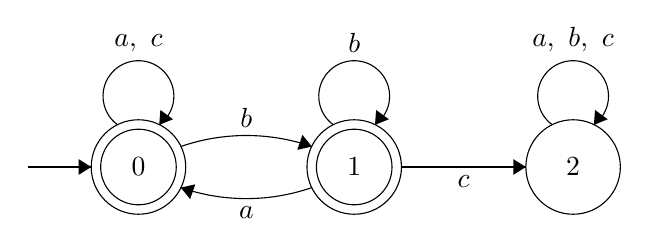
\begin{tikzpicture}[scale=0.2]
\tikzstyle{every node}+=[inner sep=0pt]
\draw [black] (23.4,-21.5) circle (3);
\draw (23.4,-21.5) node {$0$};
\draw [black] (23.4,-21.5) circle (2.4);
\draw [black] (37.1,-21.5) circle (3);
\draw (37.1,-21.5) node {$1$};
\draw [black] (37.1,-21.5) circle (2.4);
\draw [black] (51,-21.5) circle (3);
\draw (51,-21.5) node {$2$};
\draw [black] (22.077,-18.82) arc (234:-54:2.25);
\draw (23.4,-14.25) node [above] {$a,\mbox{ }c$};
\fill [black] (24.72,-18.82) -- (25.6,-18.47) -- (24.79,-17.88);
\draw [black] (26.095,-20.197) arc (109.05152:70.94848:12.73);
\fill [black] (34.41,-20.2) -- (33.81,-19.46) -- (33.49,-20.41);
\draw (30.25,-19) node [above] {$b$};
\draw [black] (35.777,-18.82) arc (234:-54:2.25);
\draw (37.1,-14.25) node [above] {$b$};
\fill [black] (38.42,-18.82) -- (39.3,-18.47) -- (38.49,-17.88);
\draw [black] (40.1,-21.5) -- (48,-21.5);
\fill [black] (48,-21.5) -- (47.2,-21) -- (47.2,-22);
\draw (44.05,-22) node [below] {$c$};
\draw [black] (49.677,-18.82) arc (234:-54:2.25);
\draw (51,-14.25) node [above] {$a,\mbox{ }b,\mbox{ }c$};
\fill [black] (52.32,-18.82) -- (53.2,-18.47) -- (52.39,-17.88);
\draw [black] (34.407,-22.807) arc (-70.87812:-109.12188:12.691);
\fill [black] (26.09,-22.81) -- (26.68,-23.54) -- (27.01,-22.6);
\draw (30.25,-24.01) node [below] {$a$};
\draw [black] (16.4,-21.5) -- (20.4,-21.5);
\fill [black] (20.4,-21.5) -- (19.6,-21) -- (19.6,-22);
\end{tikzpicture}
\newline
\end{center}

حال آن را به خودكاره غيرقطعی متناهی گسترش يافته تبدیل می‌کنیم. برای این کار یک استیت شروع و پایان جدید اضافه می‌نماییم و مطابق جزئیات گفته شده در اسلایدها ادامه می‌دهیم:

\begin{center}
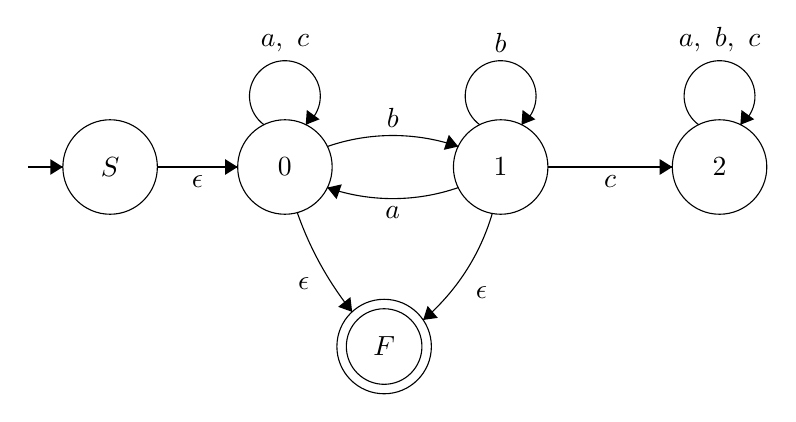
\begin{tikzpicture}[scale=0.2]
\tikzstyle{every node}+=[inner sep=0pt]
\draw [black] (23.4,-21.5) circle (3);
\draw (23.4,-21.5) node {$0$};
\draw [black] (37.1,-21.5) circle (3);
\draw (37.1,-21.5) node {$1$};
\draw [black] (51,-21.5) circle (3);
\draw (51,-21.5) node {$2$};
\draw [black] (12.3,-21.5) circle (3);
\draw (12.3,-21.5) node {$S$};
\draw [black] (29.7,-32.9) circle (3);
\draw (29.7,-32.9) node {$F$};
\draw [black] (29.7,-32.9) circle (2.4);
\draw [black] (22.077,-18.82) arc (234:-54:2.25);
\draw (23.4,-14.25) node [above] {$a,\mbox{ }c$};
\fill [black] (24.72,-18.82) -- (25.6,-18.47) -- (24.79,-17.88);
\draw [black] (26.095,-20.197) arc (109.05152:70.94848:12.73);
\fill [black] (34.41,-20.2) -- (33.81,-19.46) -- (33.49,-20.41);
\draw (30.25,-19) node [above] {$b$};
\draw [black] (35.777,-18.82) arc (234:-54:2.25);
\draw (37.1,-14.25) node [above] {$b$};
\fill [black] (38.42,-18.82) -- (39.3,-18.47) -- (38.49,-17.88);
\draw [black] (40.1,-21.5) -- (48,-21.5);
\fill [black] (48,-21.5) -- (47.2,-21) -- (47.2,-22);
\draw (44.05,-22) node [below] {$c$};
\draw [black] (49.677,-18.82) arc (234:-54:2.25);
\draw (51,-14.25) node [above] {$a,\mbox{ }b,\mbox{ }c$};
\fill [black] (52.32,-18.82) -- (53.2,-18.47) -- (52.39,-17.88);
\draw [black] (34.407,-22.807) arc (-70.87812:-109.12188:12.691);
\fill [black] (26.09,-22.81) -- (26.68,-23.54) -- (27.01,-22.6);
\draw (30.25,-24.01) node [below] {$a$};
\draw [black] (7.1,-21.5) -- (9.3,-21.5);
\fill [black] (9.3,-21.5) -- (8.5,-21) -- (8.5,-22);
\draw [black] (15.3,-21.5) -- (20.4,-21.5);
\fill [black] (20.4,-21.5) -- (19.6,-21) -- (19.6,-22);
\draw (17.85,-22) node [below] {$\epsilon$};
\draw [black] (27.669,-30.696) arc (-141.36341:-160.78373:21.348);
\fill [black] (27.67,-30.7) -- (27.56,-29.76) -- (26.78,-30.38);
\draw (24.99,-28.89) node [left] {$\epsilon$};
\draw [black] (36.568,-24.447) arc (-16.33189:-49.64515:14.075);
\fill [black] (32.18,-31.21) -- (33.11,-31.08) -- (32.46,-30.32);
\draw (35.49,-29.47) node [right] {$\epsilon$};
\end{tikzpicture}
\newline
\end{center}

استیت 2 در این حالت مرده در نظر گرفته می‌شود زیرا از آن به استیت نهایی نمی‌رسیم:

\begin{center}
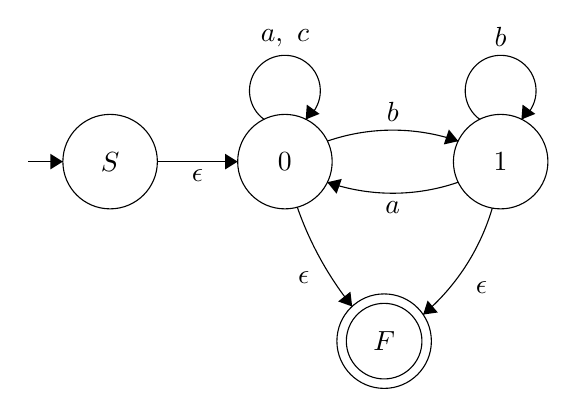
\begin{tikzpicture}[scale=0.2]
\tikzstyle{every node}+=[inner sep=0pt]
\draw [black] (23.4,-21.5) circle (3);
\draw (23.4,-21.5) node {$0$};
\draw [black] (37.1,-21.5) circle (3);
\draw (37.1,-21.5) node {$1$};
\draw [black] (12.3,-21.5) circle (3);
\draw (12.3,-21.5) node {$S$};
\draw [black] (29.7,-32.9) circle (3);
\draw (29.7,-32.9) node {$F$};
\draw [black] (29.7,-32.9) circle (2.4);
\draw [black] (22.077,-18.82) arc (234:-54:2.25);
\draw (23.4,-14.25) node [above] {$a,\mbox{ }c$};
\fill [black] (24.72,-18.82) -- (25.6,-18.47) -- (24.79,-17.88);
\draw [black] (26.095,-20.197) arc (109.05152:70.94848:12.73);
\fill [black] (34.41,-20.2) -- (33.81,-19.46) -- (33.49,-20.41);
\draw (30.25,-19) node [above] {$b$};
\draw [black] (35.777,-18.82) arc (234:-54:2.25);
\draw (37.1,-14.25) node [above] {$b$};
\fill [black] (38.42,-18.82) -- (39.3,-18.47) -- (38.49,-17.88);
\draw [black] (34.407,-22.807) arc (-70.87812:-109.12188:12.691);
\fill [black] (26.09,-22.81) -- (26.68,-23.54) -- (27.01,-22.6);
\draw (30.25,-24.01) node [below] {$a$};
\draw [black] (7.1,-21.5) -- (9.3,-21.5);
\fill [black] (9.3,-21.5) -- (8.5,-21) -- (8.5,-22);
\draw [black] (15.3,-21.5) -- (20.4,-21.5);
\fill [black] (20.4,-21.5) -- (19.6,-21) -- (19.6,-22);
\draw (17.85,-22) node [below] {$\epsilon$};
\draw [black] (27.669,-30.696) arc (-141.36341:-160.78373:21.348);
\fill [black] (27.67,-30.7) -- (27.56,-29.76) -- (26.78,-30.38);
\draw (24.99,-28.89) node [left] {$\epsilon$};
\draw [black] (36.568,-24.447) arc (-16.33189:-49.64515:14.075);
\fill [black] (32.18,-31.21) -- (33.11,-31.08) -- (32.46,-30.32);
\draw (35.49,-29.47) node [right] {$\epsilon$};
\end{tikzpicture}
\newline
\end{center}

اکنون استیت 1 را حذف می‌نماییم:

\begin{center}
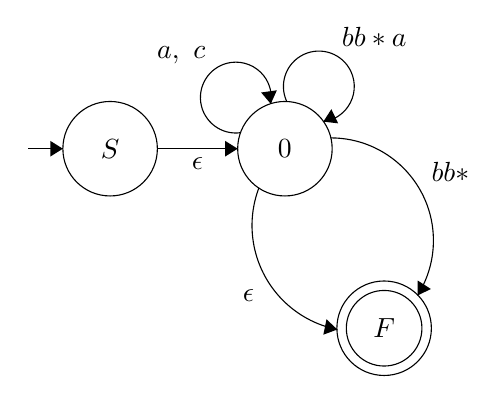
\begin{tikzpicture}[scale=0.2]
\tikzstyle{every node}+=[inner sep=0pt]
\draw [black] (23.4,-21.5) circle (3);
\draw (23.4,-21.5) node {$0$};
\draw [black] (12.3,-21.5) circle (3);
\draw (12.3,-21.5) node {$S$};
\draw [black] (29.7,-32.9) circle (3);
\draw (29.7,-32.9) node {$F$};
\draw [black] (29.7,-32.9) circle (2.4);
\draw [black] (20.59,-20.482) arc (277.82286:-10.17714:2.25);
\draw (16.82,-16.15) node [above] {$a,\mbox{ }c$};
\fill [black] (22.5,-18.65) -- (22.89,-17.79) -- (21.89,-17.93);
\draw [black] (7.1,-21.5) -- (9.3,-21.5);
\fill [black] (9.3,-21.5) -- (8.5,-21) -- (8.5,-22);
\draw [black] (15.3,-21.5) -- (20.4,-21.5);
\fill [black] (20.4,-21.5) -- (19.6,-21) -- (19.6,-22);
\draw (17.85,-22) node [below] {$\epsilon$};
\draw [black] (26.726,-32.978) arc (-101.27018:-200.87697:6.732);
\fill [black] (26.73,-32.98) -- (26.04,-32.33) -- (25.84,-33.31);
\draw (21.48,-30.83) node [left] {$\epsilon$};
\draw [black] (23.522,-18.514) arc (205.38954:-82.61046:2.25);
\draw (29.07,-15.07) node [above] {$bb*a$};
\fill [black] (25.84,-19.78) -- (26.78,-19.89) -- (26.35,-18.99);
\draw [black] (26.293,-20.813) arc (90.16987:-32.31701:6.518);
\fill [black] (31.82,-30.82) -- (32.67,-30.41) -- (31.83,-29.87);
\draw (32.68,-22.98) node [right] {$bb*$};
\end{tikzpicture}
\newline
\end{center}

حال تنها استیت باقی‌مانده یعنی 0 را حذف می‌نماییم. قبل آن کمی ساده می‌کنیم:

\begin{center}
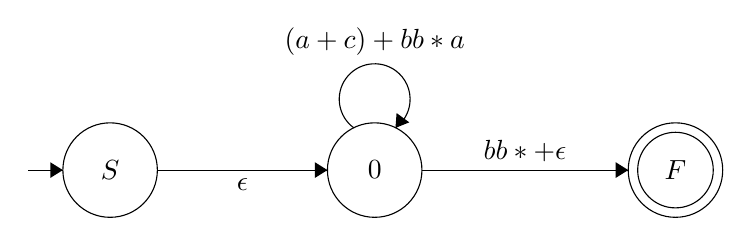
\begin{tikzpicture}[scale=0.2]
\tikzstyle{every node}+=[inner sep=0pt]
\draw [black] (29.1,-21.5) circle (3);
\draw (29.1,-21.5) node {$0$};
\draw [black] (12.3,-21.5) circle (3);
\draw (12.3,-21.5) node {$S$};
\draw [black] (48.2,-21.5) circle (3);
\draw (48.2,-21.5) node {$F$};
\draw [black] (48.2,-21.5) circle (2.4);
\draw [black] (7.1,-21.5) -- (9.3,-21.5);
\fill [black] (9.3,-21.5) -- (8.5,-21) -- (8.5,-22);
\draw [black] (15.3,-21.5) -- (26.1,-21.5);
\fill [black] (26.1,-21.5) -- (25.3,-21) -- (25.3,-22);
\draw (20.7,-22) node [below] {$\epsilon$};
\draw [black] (27.777,-18.82) arc (234:-54:2.25);
\draw (29.1,-14.25) node [above] {$(a+c)+bb*a$};
\fill [black] (30.42,-18.82) -- (31.3,-18.47) -- (30.49,-17.88);
\draw [black] (32.1,-21.5) -- (45.2,-21.5);
\fill [black] (45.2,-21.5) -- (44.4,-21) -- (44.4,-22);
\draw (38.65,-21) node [above] {$bb*+\epsilon$};
\end{tikzpicture}
\newline
\end{center}

و در مرحله آخر داریم:

\begin{center}
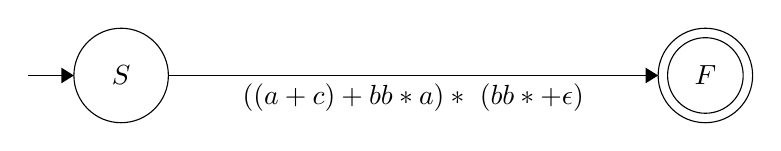
\begin{tikzpicture}[scale=0.2]
\tikzstyle{every node}+=[inner sep=0pt]
\draw [black] (18.4,-34.4) circle (3);
\draw (18.4,-34.4) node {$S$};
\draw [black] (55.5,-34.4) circle (3);
\draw (55.5,-34.4) node {$F$};
\draw [black] (55.5,-34.4) circle (2.4);
\draw [black] (12.5,-34.4) -- (15.4,-34.4);
\fill [black] (15.4,-34.4) -- (14.6,-33.9) -- (14.6,-34.9);
\draw [black] (21.4,-34.4) -- (52.5,-34.4);
\fill [black] (52.5,-34.4) -- (51.7,-33.9) -- (51.7,-34.9);
\draw (36.95,-34.9) node [below] {$((a+c)+bb*a)*\mbox{ }(bb*+\epsilon)$};
\end{tikzpicture}
\newline
\end{center}

بنابراین به عبارت منظم زیر خواهیم رسید:
\begin{center}
    $(a+c+b^+a)^*\; (b^++\epsilon)$
\end{center}